% ============================================================

% HAN Model Card – Fake-News Detection

% Adapted from: Mitchell et al., “Model Cards for Model Reporting”

% ============================================================

\documentclass[11pt]{article}

\usepackage{geometry}

\geometry{margin=1in}

\usepackage{booktabs}

\usepackage{hyperref}

\usepackage{enumitem}

\usepackage{float}

\usepackage{graphicx}

\hypersetup{colorlinks=true, linkcolor=black, urlcolor=blue}

  

\title{Model Card for \textbf{HAN-FakeNews-Detector} \\[2pt]

\large (Hierarchical Attention Network for Binary Fake-News Classification)}

\author{Akziz Amin, Lema Santiago, Raj Anshu, Ziehm Leander-Arun}

\date{Model version: \texttt{v0.1} \quad Compiled: \today}

  

\begin{document}

\maketitle

  

% ------------------------------------------------------------

\section{Model Details}

\begin{itemize}[leftmargin=*, label=--]

\item \textbf{Developed by} students at the Deggendorf Institute of Technology, June~2025, v0.1.

\item \textbf{Vocabulary size at fit time}: 50\,000 tokens; minimum word frequency = 2.

\item \textbf{Architecture:} Hierarchical Attention Network comprising:

\begin{itemize}[noitemsep,topsep=0pt]

\item \emph{Input}: documents truncated to 20 sentences × 50 tokens and mapped to 200-d trainable embeddings.

\item \emph{Word encoder}: one bidirectional GRU layer (50 hidden units each direction, dropout 0.1) with 100-d additive attention.

\item \emph{Sentence encoder}: one bidirectional GRU layer (50 hidden units each direction, dropout 0.1) with 100-d attention.

\item \emph{Classifier}: 100-d document vector → fully connected layer → two logits.

\end{itemize}

\end{itemize}

  

% ------------------------------------------------------------

\section{Intended Use}

\subsection*{Primary intended uses}

Assist fact-checkers, journalists and platform moderators by flagging news articles likely to be fabricated or misleading.

  

\subsection*{Primary intended users}

Media-monitoring organisations, newsroom editors, social-media trust \& safety teams, researchers studying misinformation.

  

\subsection*{Out-of-scope uses}

\begin{itemize}[leftmargin=*, label=--]

\item Fully autonomous removal or down-ranking of content without human review.

\item Real-time moderation of live audio/video streams.

\item Legal or policy enforcement decisions without corroborating evidence.

\end{itemize}

  

% ------------------------------------------------------------

\section{Factors}

\begin{itemize}[leftmargin=*, label=--]

\item \textbf{Language}: English-only; performance may drop on other languages or heavy dialect.

\item \textbf{Domain}: politics, health, celebrity gossip etc.~have different linguistic cues.

\item \textbf{Article length}: short posts $<$100 words often truncated to one or two sentences.

\item \textbf{Publication date}: model frozen on 2018 data; concept drift likely as new rumours emerge.

\end{itemize}

  

% ------------------------------------------------------------

\section{Metrics}

\begin{itemize}[leftmargin=*, label=--]

\item Accuracy, Precision, Recall, F1, AUROC, Average Precision.

\item Threshold 0.50 (equal-error point on validation ROC).

\item Uncertainty: 95\,\% CI from 100-round bootstrap on the test split.

\end{itemize}

  

\begin{table}[H]

\centering

\caption{Aggregate performance (stratified 80/10/10 split).}

\begin{tabular}{lccccc}

\toprule

Split & Accuracy & Precision & Recall & F1 & AUROC \\

\midrule

Validation & 0.9993 & 0.9993 & 0.9993 & 0.9993 & 1.0000 \\

Test & 0.9984 & 0.9984 & 0.9984 & 0.9984 & 0.9999 \\

\bottomrule

\end{tabular}

\end{table}

  

\textit{Robustness checks.}

5-fold CV mean $\pm$ SD: Acc.\,$=0.9988 \pm 0.0004$;

bootstrap 95\,\% CI: Acc.\,$=0.9985\,[0.9971,\,0.9996]$, AUROC\,$=0.9999\,[0.9998,\,1.0000]$.

  

\begin{figure}[H]

\centering

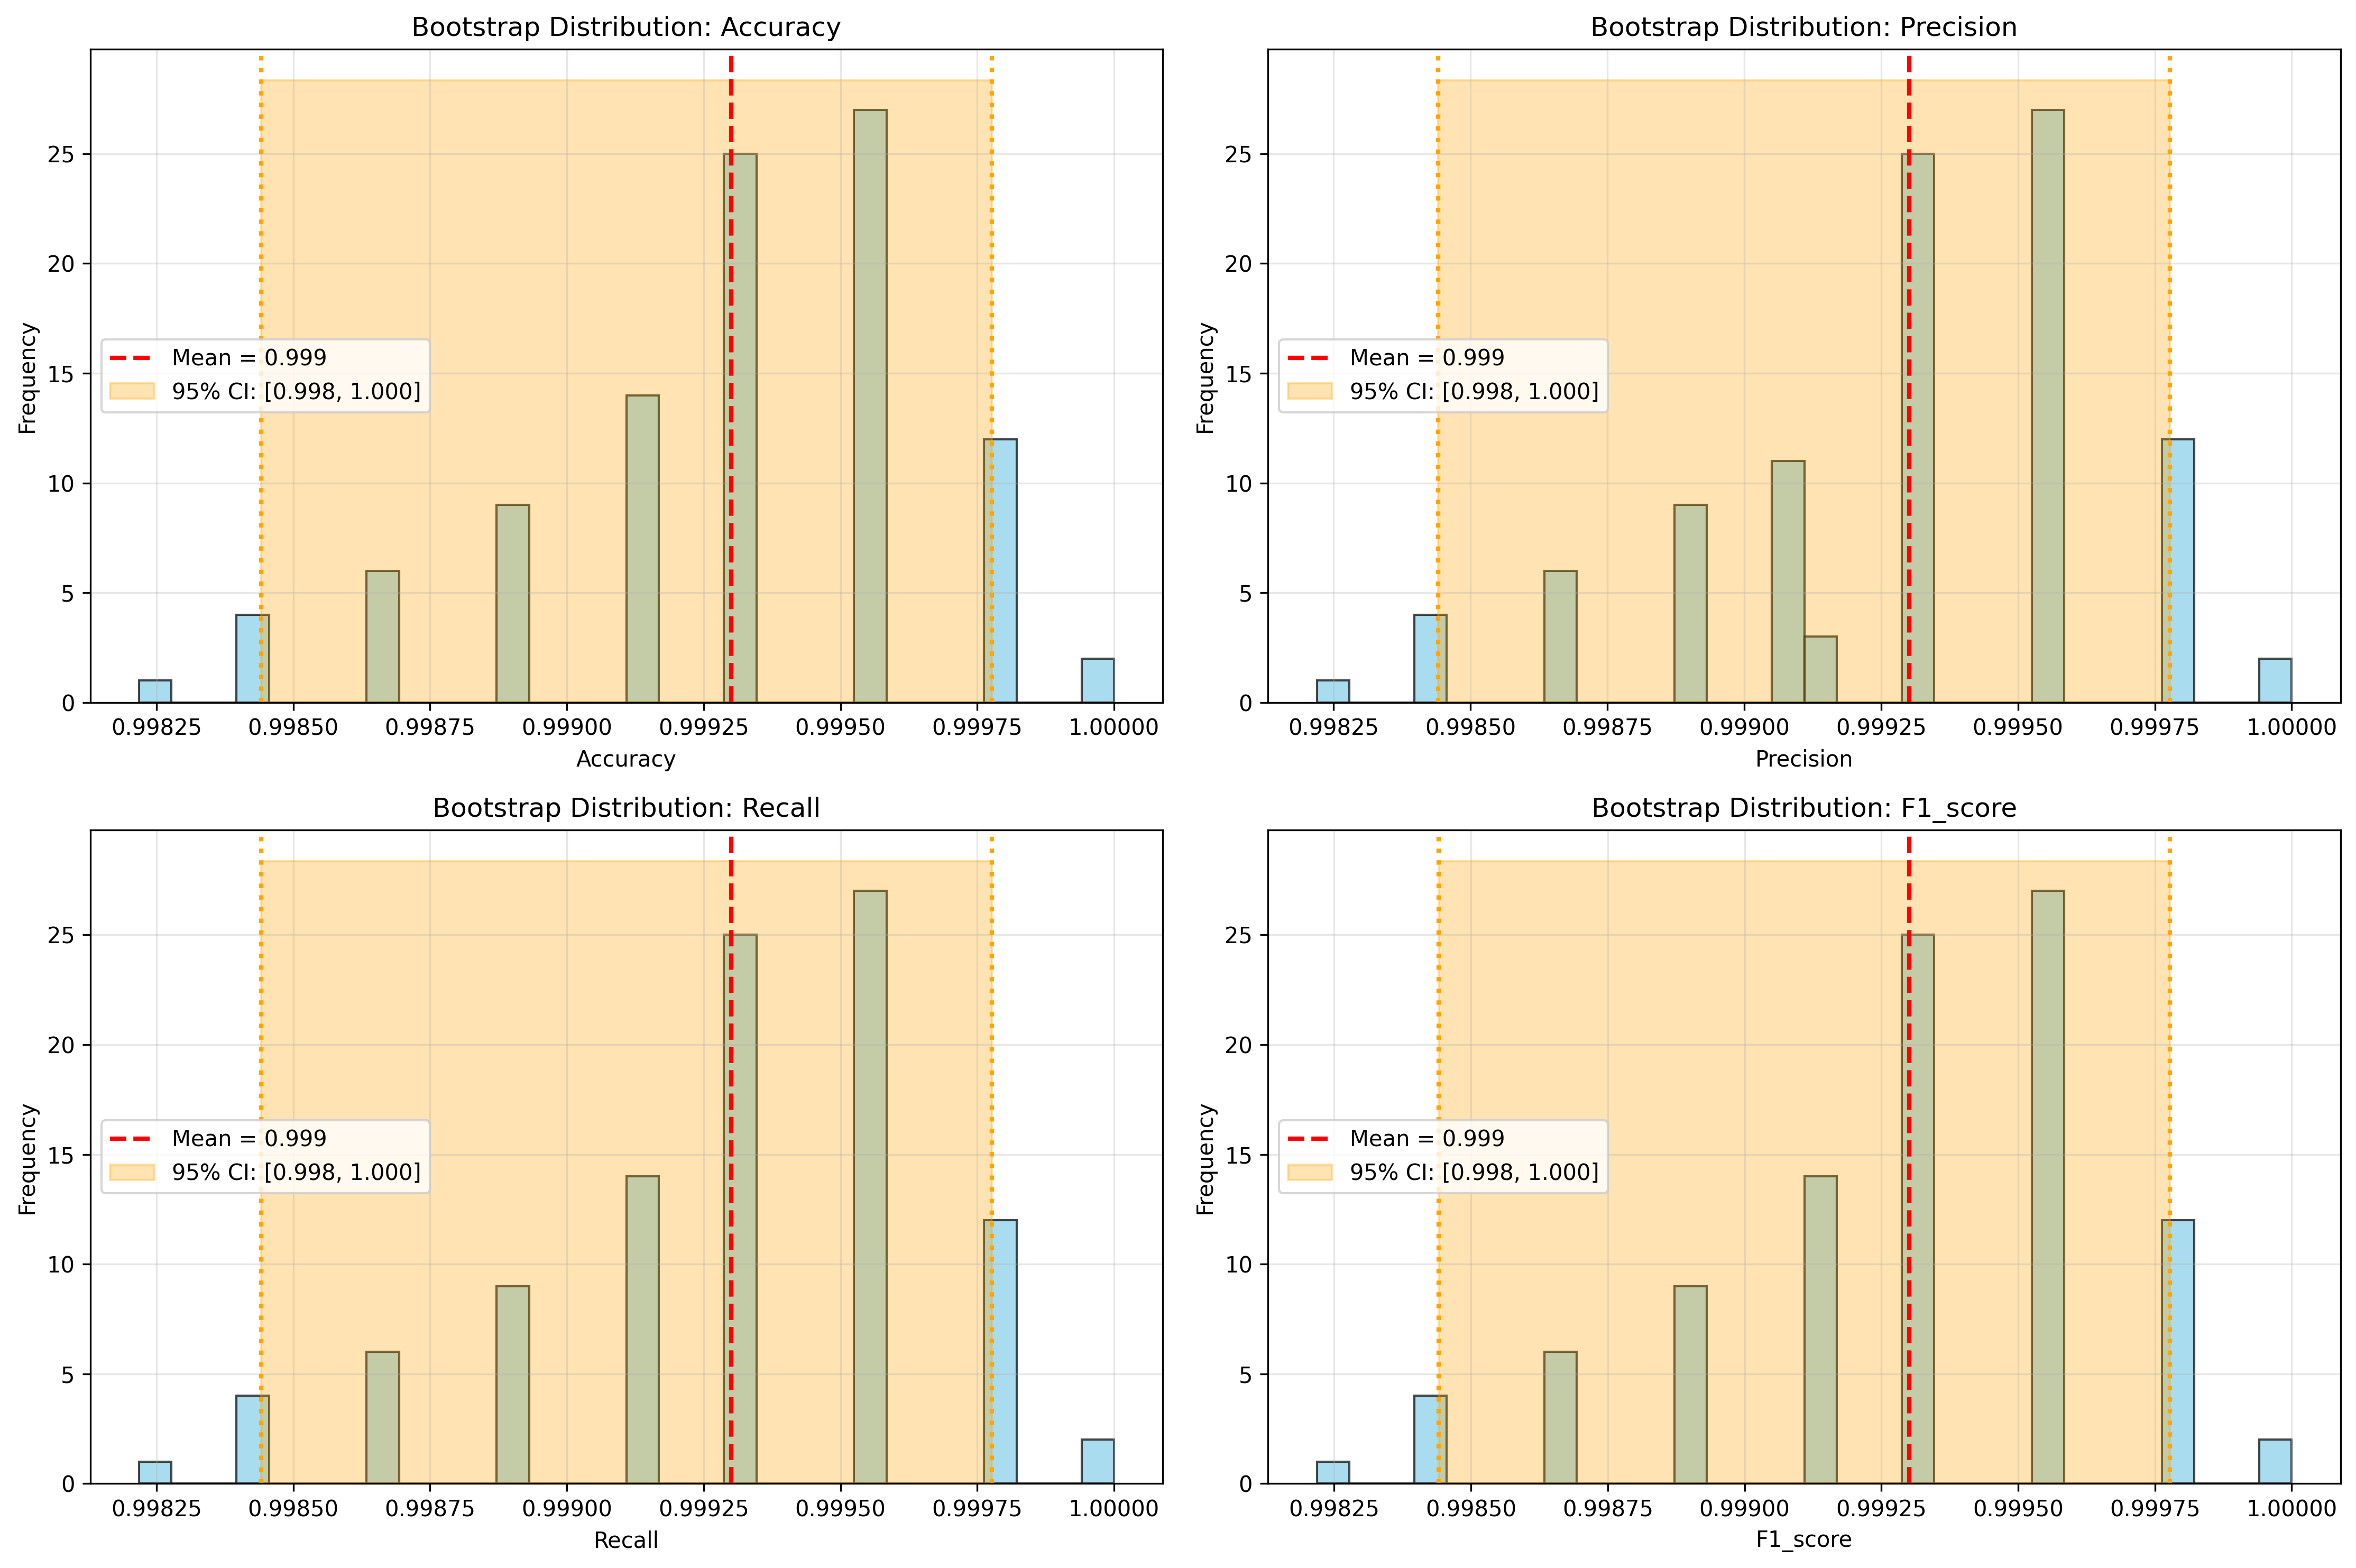
\includegraphics[width=0.8\linewidth]{../plots/bootstrap_distributions.png}

\caption{Bootstrap distribution of key metrics.}

\end{figure}

  

% ------------------------------------------------------------

\section{Training Data}

\begin{itemize}[leftmargin=*, label=--]

\item \textbf{Source}: Kaggle \texttt{Fake.csv} and \texttt{True.csv}.

\item \textbf{Size}: 45\,898 articles (fake 23\,481, true 22\,417).

\item \textbf{Splits (stratified)}: Train 35\,918, Validation 4\,490, Test 4\,490.

\item \textbf{Pre-processing}: lower-casing, punctuation kept, NLTK tokenisation; truncation to 20×50; words $<$2 occurrences mapped to \texttt{<UNK>}.

\end{itemize}

  

% ------------------------------------------------------------

\section{Evaluation Data}

Same schema as training set.

Held-out test split never used for hyper-parameter tuning.

Additional robustness: 5-fold cross-validation and 100-round bootstrap.

  

% ------------------------------------------------------------

\section{Ethical Considerations}

\begin{itemize}[leftmargin=*, label=--]

\item Possible false-positives on satire or opinion pieces.

\item Label bias in the original dataset propagates to predictions.

\item Drift: new misinformation styles may reduce recall over time.

\item Mitigations: periodic re-training, human-in-the-loop review, external bias audits.

\end{itemize}

  

% ------------------------------------------------------------

\section{Caveats \& Recommendations}

\begin{itemize}[leftmargin=*, label=--]

\item Not optimised for micro-posts ($<$20 tokens).

\item Retrain every 3–6 months to counter concept drift.

\item For multilingual deployment start with multilingual embeddings and fine-tune.

\end{itemize}

  

% ------------------------------------------------------------

\end{document}